En esta secci\'on se presentan algunos ej\'emplos de programas con el resultado correspondiente.

\subsection{Programas v\'alidos}

\lstinputlisting[breaklines=true]{../Ejemplos/eg04.peg}

\centerline{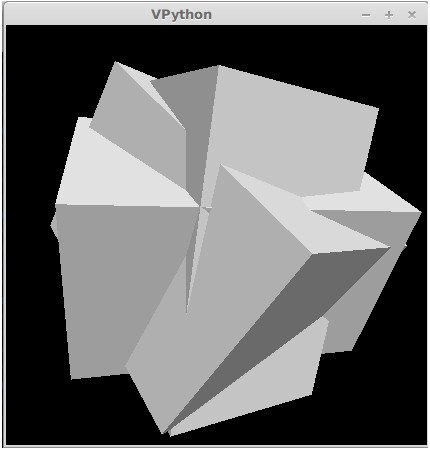
\includegraphics[scale=0.40]{../imagenes/eg04.jpg}}



\lstinputlisting[breaklines=true]{../Ejemplos/eg11.peg}

\centerline{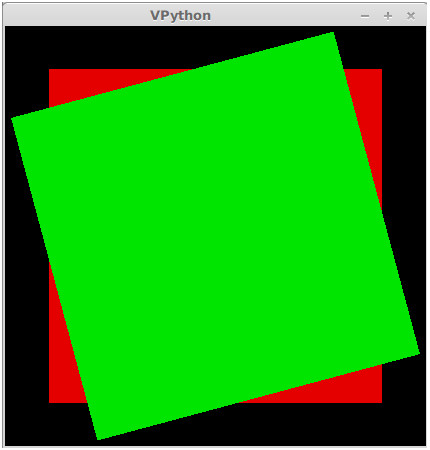
\includegraphics[scale=0.40]{../imagenes/eg11.jpg}}




\lstinputlisting[breaklines=true]{../Ejemplos/eg22.peg}

\centerline{
\includegraphics[scale=0.40]{../imagenes/eg22.png}}


\lstinputlisting[breaklines=true]{../Ejemplos/eg23.peg}

\centerline{
\includegraphics[scale=0.40]{../imagenes/eg23.png}}



\lstinputlisting[breaklines=true]{../Ejemplos/eg24.peg}

\centerline{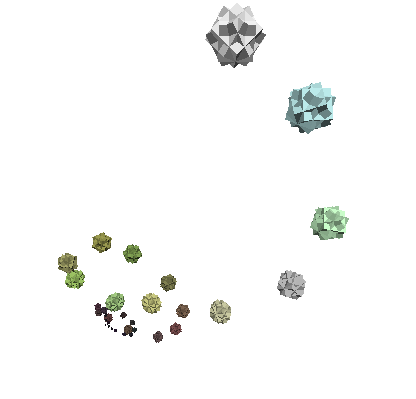
\includegraphics[scale=0.40]{../imagenes/eg24.png}}


\lstinputlisting[breaklines=true]{../Ejemplos/eg25.peg}

\centerline{
\includegraphics[scale=0.40]{../imagenes/eg25.png}}


\lstinputlisting[breaklines=true]{../Ejemplos/eg26.peg}

\centerline{
\includegraphics[scale=0.40]{../imagenes/eg26.png}}


\lstinputlisting[breaklines=true]{../Ejemplos/eg27.peg}

\centerline{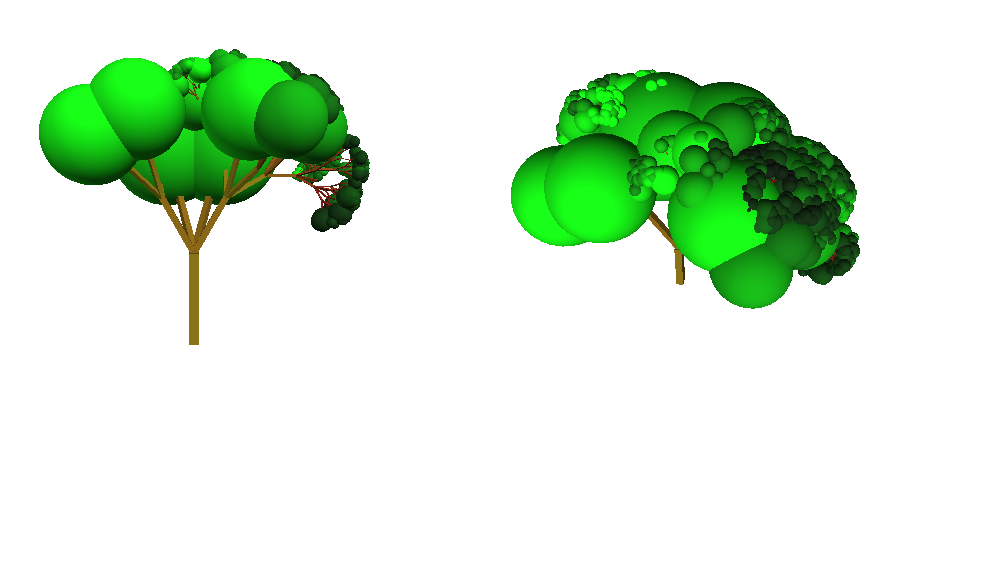
\includegraphics[scale=0.40]{../imagenes/eg27.png}}


\newpage

\subsection{Programas inv\'alidos}

\lstinputlisting[breaklines=true]{../Ejemplos/eg22invalid.peg}

\centerline{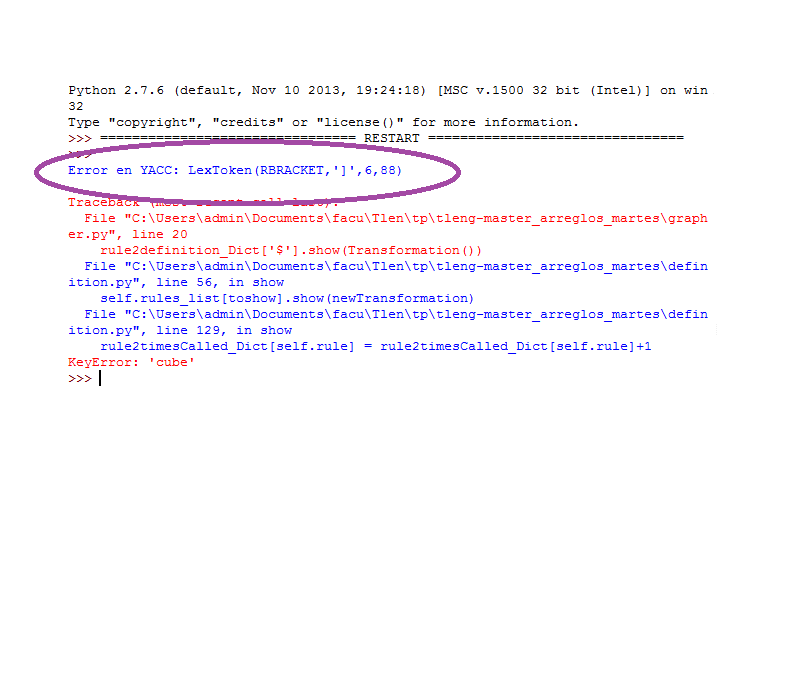
\includegraphics[scale=0.40]{../imagenes/eg22invalid.png}}

\lstinputlisting[breaklines=true]{../Ejemplos/eg22invalid2.peg}

\centerline{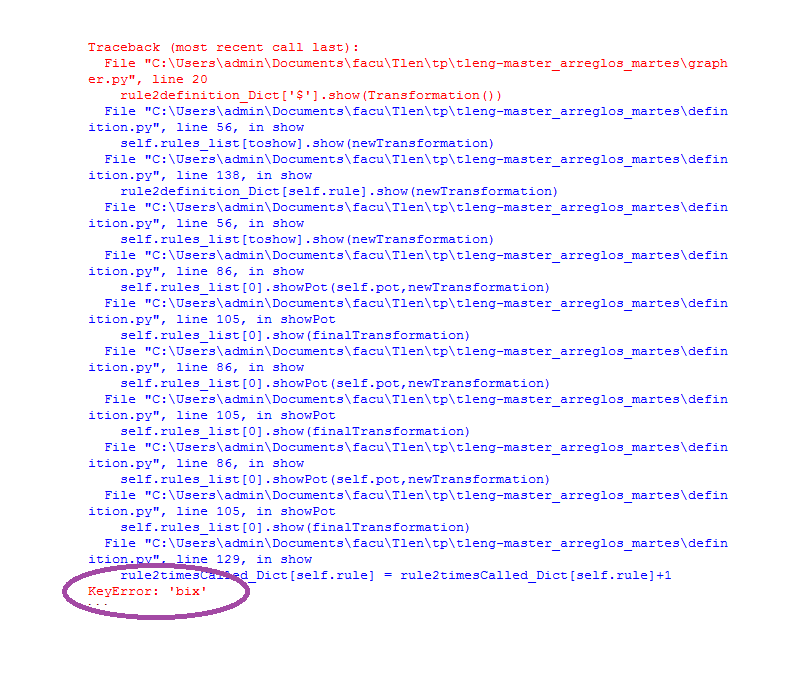
\includegraphics[scale=0.40]{../imagenes/eg22invalid2.png}}
